\section{Introduction}

Repeat what was in the intro a bit

Why do this?

say something about \texttt{mmds}


Do I need to say something about Len here?


%%%%%%%%%%%%%%%%%%%%%%%%%%%%%%%%%%%%%%%%%%%%%%%%%%%
\section{General formulation}

This section lays out, mathematically, the mixture model formulations that can be used for distance sampling detection functions. Beginning with the simplest case (line transects with no covariates) the models are built up and it is shown that the simpler models are just special cases of the more complex ones, thus providing a general framework for mixture model detection functions.

The core principle here is to replace the ``key function plus adjustment terms'' model for the detection function with a mixture model. The simplest example would be to define $g$ as some finite weighted sum of $J$ half-Normal distributions:
\begin{equation}
g(x;\bm{\sigma},\bm{\pi}) = \sum_{j=1}^J \pi_j \exp \Big( \frac{-x^2}{2 \sigma_j^2}\Big).
\label{mmds-simplemix}
\end{equation}
Where the mixture proportions, $\pi_j$, have the property $\sum_{\forall j}\pi_j=1$ and $\bm{\pi} = (\pi_1, \dots, \pi_J)$. $\bm{\sigma}=(\sigma_1,\sigma_2,\dots,\sigma_J)$ are scale parameters. An example of a 2-point mixture of half-Normals is given in figure \ref{2ptdia}.

\begin{figure}
\centering
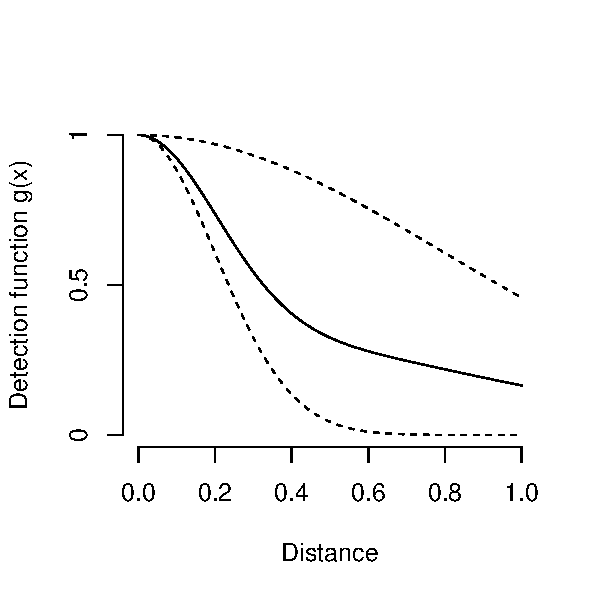
\includegraphics[width=4in]{mix/figs/2ptdia.pdf}
\caption{An example of a 2-point mixture of half-Normals. The two constituent mixture parts are shown with dashed lines, the whole mixture function is the solid line. The scale parameters for the Normal distributions are $0.8$ and $0.2$. The associated mixture proportions are $0.64$ and $0.36$.}
\label{2ptdia}
\end{figure}

Clearly one can think of more complex versions of this: different functions, continuous mixtures or a finite mixture of continuous and finite mixtures (\textit{a la} \cite{morgan08}). However, here only the finite mixture case with half-Normal key functions is considered.

\subsection{Line transects}
For line transects, we can simply substitute equation (\ref{mmds-simplemix}) into the line transect likelihood in equation (\ref{ds-lt-likelihood}). Before doing this we first note that the definition of $\mu$ has not changed, merely the definition of $g$:
\begin{align*}
\mu = \int_0^w \sum_{j=1}^J \pi_j g_j(x;\sigma_j) \text{d}x = \sum_{j=1}^J \pi_j \int_0^w  g_j(x;\sigma_j) \text{d}x = \sum_{j=1}^J \pi_j \mu_j.
\end{align*}
So, the likelihood becomes:
\begin{align}
\mathcal{L}(\bm{\sigma}, \bm{\pi}; \bm{x}) &= \prod_{i=1}^n f(x_i;\bm{\sigma}, \bm{\pi}),\\
&= \prod_{i=1}^n \frac{g(x_i;\bm{\sigma}, \bm{\pi})}{\mu},\\
&= \prod_{i=1}^n \frac{\sum_{j=1}^J \pi_j \exp \Big( \frac{-x_i^2}{2 \sigma_j^2}\Big)}{\sum_{j=1}^J \pi_j \int_0^w  g_j(x;\sigma_j) \text{d}x}.
\label{mmds-lt-likelihood}
\end{align}
which we can obviously think of alternatively as:
\begin{align}
\mathcal{L}(\bm{\sigma}, \bm{\pi}; \bm{x}) &= \prod_{i=1}^n f(x_i;\bm{\sigma}, \bm{\pi}),\\
&= \prod_{i=1}^n \sum_{j=1}^J \pi_j f_j(x_i;\bm{\sigma}, \bm{\pi}),\\
&= \prod_{i=1}^n \sum_{j=1}^J \pi_j \frac{\exp \Big( \frac{-x_i^2}{2 \sigma_j^2}\Big)}{\int_0^w  g_j(x;\sigma_j) \text{d}x}.
\label{mmds-lt-likelihood-pdf}
\end{align}

\subsection{Point transects}
The detection function is, of course, the same for point transects as for line transects. What changes is the PDF and hence likelihood. The likelihood is therefore given as:
\begin{align}
\mathcal{L}(\bm{\sigma}, \bm{\pi}; \bm{r}) &= \prod_{i=1}^n f(r_i;\bm{\sigma}, \bm{\pi}),\\
&= \prod_{i=1}^n \sum_{j=1}^J \pi_j f_j(r_i;\bm{\sigma}, \bm{\pi}),\\
&= \prod_{i=1}^n \sum_{j=1}^J \pi_j \frac{r_i \exp \Big( \frac{-r_i^2}{2 \sigma_j^2}\Big)}{\int_0^w r  g_j(r;\sigma_j) \text{d}r}.
\label{mmds-pt-likelihood-pdf}
\end{align}
where we can define a per-mixture effective area of detection:
\begin{equation}
\nu_j=\int_0^w r  g_j(r;\sigma_j) \text{d}r,
\end{equation}
which is analogous to $\mu_j$, above.

Having these two likelihoods written down, the formulation for covariate models and the generalised likelihood can be derived.

\subsection{Covariate models}
The above models show that the differences between the CDS and mixture model DS (MMDS) are fairly minimal. For the covariate case things are a little more tricky. There are many possible model formulations and the notation is therefore more complicated.

For simplicity of notation, we consider the case where one distance, $x$ (alternatively $r$ for point transects), has been observed and a set of corresponding covariates $z_1,\dots,z_K$ have been recorded too. As before $\sigma_j$ is a (link) function of these covariates and a set of coefficients, the detection function is then defined as:
\begin{equation*}
g(x, \bm{z};\bm{\beta},\bm{\pi}) = \sum_{j=1}^J \pi_j \exp \Big( \frac{-x^2}{2 \sigma_j(\bm{z};\bm{\beta}_j)^2}\Big),
\end{equation*}
defining $\sigma_j(\bm{z};\bm{\beta}_j)$ to be,
\begin{equation*}
\sigma_j(\bm{z};\bm{\beta}_j) = \exp \Big(\beta_{0j} + \sum_{k\in K_j} \beta_{kj} z_k \Big),
\end{equation*}
where $\bm{z}$ is the $K$-vector of all covariates. $K_j$ is the set of covariates to be used with mixture $j$. The vector of per mixture coefficients is $\bm{\beta}_j=(\beta_{0j},\{ \beta_{kj} : k \in K_j\})$. Finally $\bm{\beta}=(\bm{\beta}_1,\dots,\bm{\beta}_J)$ is the vector of all coefficients ordered by mixture part then covariate.

When we have multiple observations we store the distances in $\bm{x}$ (an $n$-vector). Then, for each observation we have a $\bm{z}_i$ and $Z$ is an $n \cross K$ matrix of the covariates for each observation (ie. the $\bm{z}_i$s stacked on top of each other. So then $z_{ik}$ would be the $i^\text{th}$ observation's covariate $k$ (and the $ik^\text{th}$ element of $Z$).

\subsubsection{Covariates - intercept model}

One can think of a special case of the model above when the parameters estimated are common across all mixture parts, except for an intercept.  Mathematically,
\begin{align*}
\sigma_j(\bm{z};\bm{\beta}_j) = \exp \Big(\beta_{0j} + \sum_{k\in K_j} \beta_{k} z_k \Big)
\end{align*}
so the $\beta_{0j}$s are estimated in each mixture but the $\beta_{k}$s are common to all mixtures and are estimated simultaneously. In this case, the $K_j$s are the same for all mixture components.

NOT CURRENTLY IMPLEMENTED

\subsection{Generalised likelihood}
\label{ds-genlik}

\subsubsection{Line transects}
Considering the non-covariate case as a special case of the covariate model, the likelihood can then be written as:
\begin{align}
\mathcal{L}(\bm{\beta}, \bm{\pi} ; \bm{x}, Z) &= \prod_{i=1}^n f(x_i;\bm{\sigma}(\bm{\beta},Z)),\\
&= \prod_{i=1}^n \frac{g(x_i;\bm{\sigma}(\bm{\beta},Z))}{\mu(Z)},\\
&= \prod_{i=1}^n \sum_{j=1}^J \pi_j \frac{g_j(x_i; \sigma_j(\bm{z}_i;\bm{\beta}_j))}{ \mu_j(\bm{z}_i)}.
\label{mmds-lt-glikelihood}
\end{align}
where the $\sigma_j(\bm{z}_i;\bm{\beta}_j)$s take the covariate form above; in the case of a no covariate model, there is only the intercept term, $\beta_{0j}$ ie:
\begin{equation}
\sigma_j = \exp ( \beta_{0j} ).
\end{equation}

\subsubsection{Point transects}
For point transects the likelihood is similar, though with the $r$ pre-multiplier as seen for CDS and MCDS:
\begin{align}
\mathcal{L}(\bm{\beta}, \bm{\pi} ; \bm{r}, Z) &= \prod_{i=1}^n f(r_i;\bm{\sigma}(\bm{\beta},Z)),\\
&= \prod_{i=1}^n \frac{g(r_i;\bm{\sigma}(\bm{\beta},Z))}{\nu(Z)},\\
&= \prod_{i=1}^n \sum_{j=1}^J \pi_j \frac{g_j(r_i; \sigma_j(\bm{z}_i;\bm{\beta}_j))}{ \nu_j(\bm{z}_i)}.
\label{mmds-pt-glikelihood}
\end{align}



\subsection{Detection probability}
Calculation of $\mu_j$ (and $\nu_j$ and their covariate analogues) leads to a per-mixture (and per-observation, per-mixture) definition for the probability of detection. Although these quantities are useful (indeed, they are needed to calculate Horvitz-Thompson-type estimators of abundance), it is also useful to calculate the overall detection probability.




$P_a$, per observation $p$, Var and CV.

\subsection{Goodness of fit testing}





%%%%%%%%%%%%%%%%%%%%%%%%%%%%%%%%%%%%%%%%%%%%%%%%%%%
\section{Implementation}
This section gives detail on the implementation of MMDS, particularly those used in the \textsf{R} package \texttt{mmds}.

\subsection{Parametrisation of the scale parameters}
The parametrisation of the $\sigma_j$s given in section \ref{ds-genlik} is not only useful because it simplifies the notation in the likelihood. It also allows for unconstrained optimisation of the scale parameters in all situations. Since $\sigma_j$ must be positive, optimising a set of $\bm{\beta}_j$s on the log scale allows for the $\bm{\beta}_j$s to take values over all of $\mathbb{R}$.


\subsection{Parametrisation of the mixture proportions}
When using 2-point mixtures, the constraint that the $\pi_j$s sum to unity is enforced by definition (since $\pi_2=1-\pi_1$). However, in $J$-point mixtures when $J>2$, ensuring that the proportions sum to 1 is not guaranteed. The obvious way to get around this would be to penalise the likelihood, should the optimisation procedure propose values for the $\pi_j$s that do no comply with this condition. This is, of course, inefficient and ugly. Instead, a parametrisation is used for the mixture proportions.

Rather than estimating the $\pi_j$s, estimate $\alpha_k$s, where the relationship between the two is:
\begin{equation*}
\pi_j = F(\sum_{k=1}^j e^{\alpha_k}) - F(\sum_{k=1}^{j-1} e^{\alpha_k}) \qquad \text{for } 1\leq k \leq J-1
\end{equation*}
and
\begin{equation*}
\pi_J = 1-\sum_{j=1}^{J-1} \pi_j
\end{equation*}
where $F$ is any continuous CDF on $(0,\infty]$. Exponentiation ensures that $e^{\alpha_j}\geq0$ (so $\alpha_j$ may lie anywhere on $\mathbb{R}$ allowing unconstrained optimisation). Summing these orders the $\pi_j$s, since only offsets are estimated. Finally, using the cumulative density function ensures that the $\pi_j$s sum to $1$. In practise the $\text{Gamma}(3,2)$ CDF is (somewhat arbitrarily) used. Figure \ref{dlbpi} shows a diagram illustrating the relationship.

% illustration of the pi parametrisation - DLB's method
\begin{figure}
\centering
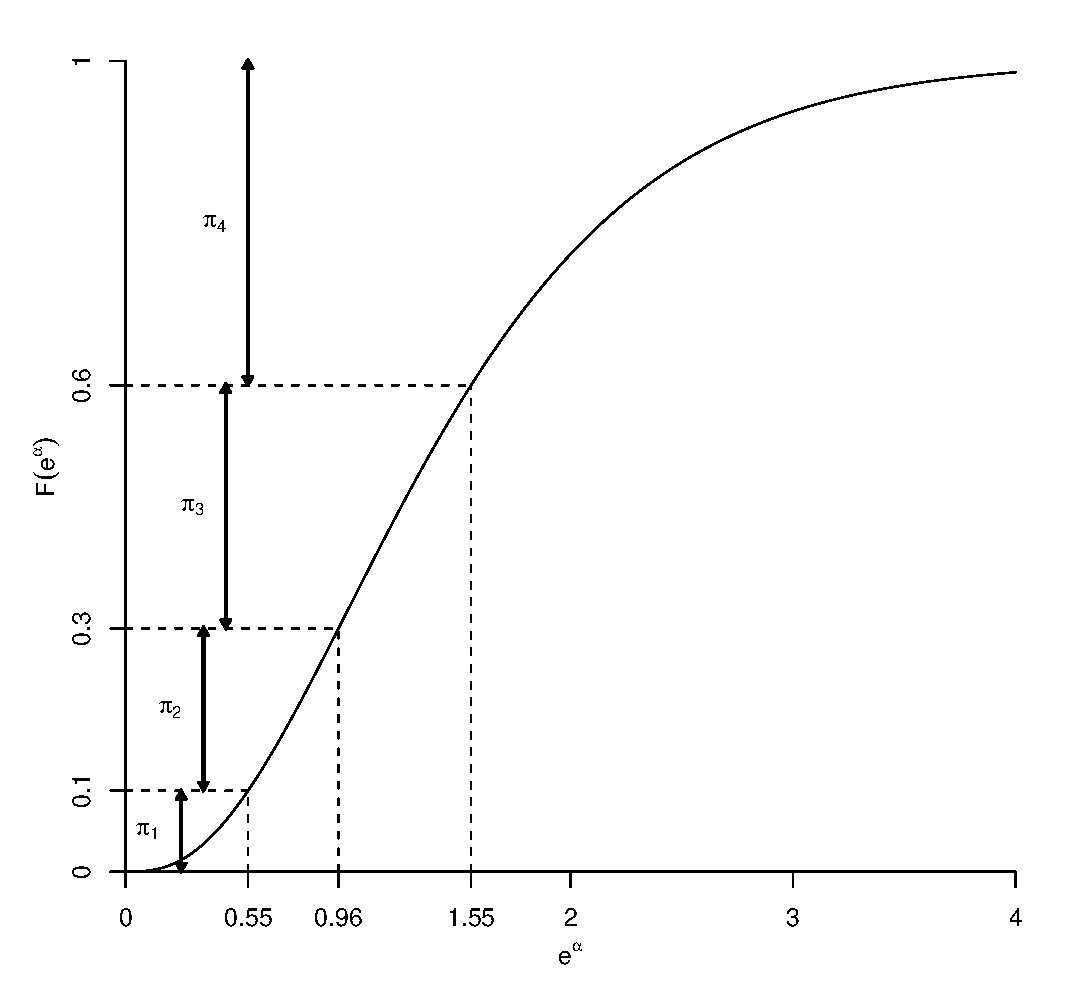
\includegraphics[width=4in]{mix/figs/pidia.pdf}
\caption{Illustration of the parameterisation of the $\pi_j$s. The black curve is a Gamma CDF (with shape parameter 3 and scale parameter 1/2). Here $\bm{\pi}=c(0.1,0.2,0.3,0.4)$. The differences in the ``heights'' of the evaluations of the CDF give the values of $\pi_j$.}
\label{dlbpi}
\end{figure}

\subsubsection{Inverse transform}
To transform from the $\pi_j$s back to the $\alpha_j$s we simply re-arrange the above expression.
\begin{align*}
\pi_j &= F(\sum_{k=1}^j e^{\alpha_k}) - F(\sum_{k=1}^{j-1} e^{\alpha_k})\\
F(\sum_{k=1}^j e^{\alpha_k}) &= \pi_j + F(\sum_{k=1}^{j-1} e^{\alpha_k})\\
\sum_{k=1}^j e^{\alpha_k} &= F^{-1}(\pi_j + F(\sum_{k=1}^{j-1} e^{\alpha_k}))\\
e^{\alpha_j} &= F^{-1}\Big(\pi_j + F(\sum_{k=1}^{j-1} e^{\alpha_k})\Big) - \sum_{k=1}^{j-1} e^{\alpha_k}\\
\alpha_j &= \log_e \Big(F^{-1}\Big(\pi_j + F(\sum_{k=1}^{j-1} e^{\alpha_k})\Big) - \sum_{k=1}^{j-1} e^{\alpha_k}\Big)
\end{align*}
Thus, it is possible to move between the two parametrisations easily.

\subsection{Fitting}
It is well known that mixture model likelihoods are notoriously multi-modal (\cite{BDA} PAGES).

MORE BLURB

Three different strategies were used for the optimisation and offered in the \texttt{mmds} package. The justification being that if one method fails to fit a particular model, then perhaps another might be better at tackling that particular problem. The first and simplest of these methods was a straightforward quasi-Newton method, BFGS (\cite{bfgs}) which simply maximised the likelihood with the help of analytic gradients (see appendix \ref{appendix-mmds-derivs}). In testing this method was unsatisfactory so two other procedures were also developed.

\subsection{BFGS+SANN}
The starting value calculation (see section \ref{mmds-starting-vals}) is relatively primitive and therefore perhaps does not start the optimisation in a particularly good position to begin the maximisation. Given this and the rather complex likelihood, the odds are not stacked in the favour of the optimisation procedure being successful. In order to move around the parameter space, simulated annealing (SIMULATED ANNEALING REF: NUM RECIPES?) is used to begin the maximisation then followed up with a BFGS step to find the maxima. Both BFGS and simulated annealing are available via the \texttt{optim()} function in the base \textsf{R} distribution.

In particular, simulated annealing is used for 250 iterations, then unconstrained BFGS after that. In an attempt to avoid local maxima, these two steps are looped for five iterations and the results stored. The model with the lowest AIC is then chosen from these. If no models fit in the first 5 iterations, the procedure continues until at least one model fits, or there have been 20 attempts at fitting, whichever comes first.

It is worth noting that the method may appear to fail to converge for all attempts, however this does not necessarily indicate that the model will never converge. The stochastic nature of simulated annealing means that it is entirely possible that further runs may yield a useful result.

\subsection{Expectation-Maximisation Algorithm}
A common (CITE SOME PAPERS) way of fitting mixture models is to use the Expectation-Maximisation (EM) algorithm of CITE THE EM PAPER.

First note that the likelihood for mixture models tends to be of the form:

this form appears to be a weighted likelihood... SAY MORE FROM THE PIATER DOC

Outline of the EM algorithm is taken from the very helpful set of notes by \cite{piater}. As is usual with EM, we loop between expectation and maximisation steps until convergence. For brevity we define:
\begin{equation*}
f_j(x_i,zj;\sigma_j) =  \frac{g_j(x_i, zj;\sigma_j)}{\mu_j(zj)},
\end{equation*}
in the line transect case and
\begin{equation*}
f_j(x_i,zj;\sigma_j) = \frac{2 \pi r_i g_j(r_i, zj;\sigma_j)}{nuj}.
\end{equation*}
for the point transect case.

\begin{itemize}
\item \textbf{Expectation}

In the expectation step we need to calculate the expected values of the $w_{ij}$ for each datum $i$ and mixture $j$,
\begin{equation*}
\mathbb{E}[w_{ij}] = \frac{\pi_j f_j(x_i,zj;\sigma_j)}{\sum_{k=1}^J \pi_k f_k(x_i,zj;\sigma_k)},
\end{equation*}
then calculate the $\pi_j$s as:
\begin{equation*}
\pi_j=\frac{1}{n} \sum_{i=1}^n w_{ij}.
\end{equation*}

\item \textbf{Maximisation}

Keeping the $\pi_j$s fixed, optimise with respect to the $\sigma_j$s (or, rather, $\beta_{jk}$s). Here we just use BFGS in \texttt{optim()}. 
\end{itemize}



cite EM/CEM/SEM paper

gelman multimodality

maybe show why other parametrisation doesn't work??


\subsection{Starting values}
\label{mmds-starting-vals}
Starting values are calculated by first sorting data by distance and then dividing it into $k$ equal parts (for a $k$ point mixture). For each of these parts work out a \cite{beavers98}-type estimate of the $\beta_{jk}$s and use that as start point. 

The Beavers and Ramsay estimate is given as the results of running an intercept only regression on $\log(x+\frac{w}{1000})$ (where $w$ denotes the truncation distance, as above) for the non-covariate models. For covariate models, the equation for the $\sigma_j$ is used. The estimated parameters from the linear regression are used as the starting values for the $\beta_{jk}s$.

For the $\alpha_j$s, a set of $\pi_j$ are generated as $1/k$ and then transformed by the procedure above to be on the $\alpha_j$ scale.



\subsection{Derivatives}
[[Maybe this is better as an appendix?]]


%%%%%%%%%%%%%%%%%%%%%%%%%%%%%%%%%%%%%%%%%%%%%%%%%%%
\section{Testing}

\subsection{Simulations}

METRICS

WHY are we doing each of these.

DISCUSSION OF (in particular)

nocovar sim 5

covar with 3pt - what's going on?

3pt with 2pt - what's going on

\subsection{Real data}

Just source in the .tex from the vignette?




%%%%%%%%%%%%%%%%%%%%%%%%%%%%%%%%%%%%%%%%%%%%%%%%%%%
\section{Conclusion}


\section{Acknowledgements}
DLB - pi parametrisation
JLL/Steve/Eric - general comments
Marc - interesting chat
Len - obviously



